\documentclass[10.5pt]{article}
\usepackage[letterpaper,margin=0.62in,headheight=16pt]{geometry}
\usepackage[T1]{fontenc}
\usepackage[utf8]{inputenc}
\usepackage{lmodern,microtype}
\usepackage{amsmath,amssymb,bm}
\usepackage{booktabs,array,tabularx,multirow}
\usepackage{siunitx}
\usepackage{xcolor}
\usepackage{tikz}
\usepackage{pgfplots}
\usepackage[most]{tcolorbox}
\usepackage{enumitem}
\usepackage{caption}
\usepackage{titlesec}
\usepackage{fancyhdr}
\usepackage{hyperref}
\usepackage{float}
\usetikzlibrary{arrows.meta,positioning,calc,fit,decorations.pathmorphing,patterns,shapes.geometric,shadows.blur,backgrounds}
\pgfplotsset{compat=1.18}
\sisetup{detect-all=true,round-mode=places,round-precision=2}

\definecolor{ink}{HTML}{111820}
\definecolor{muted}{HTML}{5C6675}
\definecolor{blueprint}{HTML}{0C63B7}
\definecolor{cyan}{HTML}{23A7D8}
\definecolor{orange}{HTML}{E08D2D}
\definecolor{green}{HTML}{2A9D63}
\definecolor{gridgray}{HTML}{D9E1EA}
\definecolor{panel}{HTML}{F6F8FB}
\definecolor{darkpanel}{HTML}{EAF0F7}
\definecolor{linegray}{HTML}{C7D1DB}

\hypersetup{colorlinks=true,linkcolor=blueprint,citecolor=blueprint,urlcolor=blueprint}
\captionsetup{font=small,labelfont=bf}
\titleformat{\section}{\Large\bfseries\color{ink}}{\thesection.}{0.5em}{}
\titleformat{\subsection}{\large\bfseries\color{ink}}{\thesubsection}{0.45em}{}
\titlespacing*{\section}{0pt}{0.9em}{0.35em}
\titlespacing*{\subsection}{0pt}{0.55em}{0.2em}
\setlist[itemize]{leftmargin=1.2em,itemsep=0.1em,topsep=0.2em}
\pagestyle{fancy}
\fancyhf{}
\lhead{Concept Technical Manuscript - Demonstration Draft}
\rhead{Four-Architecture Gravity Storage}
\cfoot{\thepage}
\renewcommand{\headrulewidth}{0.25pt}
\newcommand{\placeholder}{\textcolor{orange}{\textsc{placeholder}}}

\begin{document}

% ---------------- Title page ----------------
\begin{titlepage}
\thispagestyle{empty}
\begin{tikzpicture}[remember picture,overlay]
\fill[ink] (current page.north west) rectangle ([yshift=-1.55in]current page.north east);
\draw[blueprint,line width=1.2pt] ([xshift=0.62in,yshift=-1.68in]current page.north west) -- ([xshift=-0.62in,yshift=-1.68in]current page.north east);
\foreach \x in {0,0.35,...,8.5} {\draw[white!10,line width=0.2pt] ([xshift=\x in]current page.south west) -- ([xshift=\x in]current page.north west);}
\foreach \y in {0,0.35,...,11} {\draw[white!7,line width=0.2pt] ([yshift=\y in]current page.south west) -- ([yshift=\y in]current page.south east);}
\node[anchor=north west,text=white,font=\bfseries\Huge,align=left,text width=6.9in] at ([xshift=0.65in,yshift=-0.36in]current page.north west) {Comparative Design of Four Gravity-Based Energy Storage Architectures};
\node[anchor=north west,text=white!82,font=\Large,align=left,text width=6.9in] at ([xshift=0.65in,yshift=-1.04in]current page.north west) {with an Electromagnetic Linear Generator Subsystem};
\end{tikzpicture}

\vspace*{1.95in}
\begin{center}
{\large A. S. Khan, Student Inventor}\par
\vspace{0.8mm}
{\normalsize Concept draft for invention logbook / technical appendix}\par
\vspace{5mm}
\end{center}

\begin{tcolorbox}[enhanced,colback=panel,colframe=blueprint,boxrule=0.9pt,arc=2pt,left=7pt,right=7pt,top=6pt,bottom=6pt]
\textbf{Abstract--} Renewable generation requires storage that is durable, scalable, and explainable. This concept manuscript presents a comparative framework for four gravity-based energy storage architectures: dual-weight regeneration, variable-counterweight regeneration, buoyancy-assisted recovery, and electromagnetic linear-machine recovery. A detailed electromagnetic subsystem is developed as a direct-drive vertical generator/motor concept using a moving permanent-magnet translator, stationary windings, guide rails, position feedback, and bidirectional power electronics. The purpose of the study is not to claim that linear-machine gravity storage is new; prior work has already demonstrated dry gravity storage systems using linear electric machines. Instead, the proposed contribution is a student-scale comparative architecture study that evaluates multiple regeneration pathways under common mass-height conditions.
\end{tcolorbox}

\vspace{2mm}
\begin{tcolorbox}[enhanced,colback=orange!6,colframe=orange,boxrule=0.75pt,arc=2pt,title={Important draft status},fonttitle=\bfseries]
This is a demonstration manuscript. Architecture names, equations beyond the basic physical model, diagrams, and numerical results are provisional. Replace placeholder values with measured prototype data, simulation outputs, final invention names, and verified sources before submitting.
\end{tcolorbox}

\vfill
\begin{center}
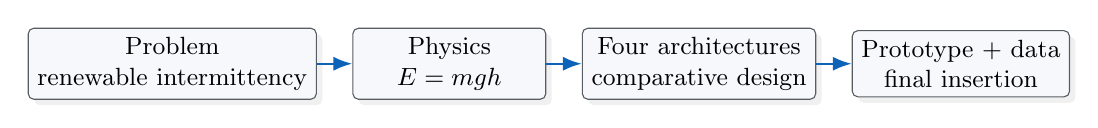
\begin{tikzpicture}[>=Latex,font=\small]
\tikzset{node/.style={draw=ink!70,fill=panel,rounded corners=2pt,minimum width=2.45cm,minimum height=0.7cm,align=center,drop shadow={opacity=0.12}},arr/.style={->,line width=0.85pt,draw=blueprint}}
\node[node] (a) {Problem\\renewable intermittency};
\node[node,right=0.45cm of a] (b) {Physics\\$E=mgh$};
\node[node,right=0.45cm of b] (c) {Four architectures\\comparative design};
\node[node,right=0.45cm of c] (d) {Prototype + data\\final insertion};
\draw[arr] (a)--(b); \draw[arr] (b)--(c); \draw[arr] (c)--(d);
\end{tikzpicture}
\end{center}
\end{titlepage}

% ---------------- Page 2 ----------------
\section{Design Objective and Prior-Art Boundary}
The project begins from the energy-storage problem: intermittent generation from solar and wind must be decoupled from consumption. Gravity storage is attractive because the storage medium can be mechanically simple: raise mass when energy is available, then recover energy during controlled descent.

\begin{equation}
E_g=m g \Delta h,
\label{eq:mgh}
\end{equation}
where $m$ is lifted mass, $g$ is gravitational acceleration, and $\Delta h$ is vertical displacement. The core design question is not merely whether gravity can store energy; the design question is which regeneration architecture makes gravity storage practical, controllable, efficient, and buildable at the desired scale.

\begin{tcolorbox}[enhanced,colback=panel,colframe=linegray,boxrule=0.5pt,arc=2pt,title={Prior-art boundary},fonttitle=\bfseries]
Published linear-machine gravity storage already exists. The reference paper by Mugyema et al. designs a \SI{130}{kW} linear electric machine for a dry gravity storage system using a \SI{100}{m} shaft and \SI{50}{ton} piston, then develops speed and current control for fast grid response. Therefore, the final project should frame the electromagnetic system as one researched architecture inside a broader four-system comparison, not as a claim that linear-machine gravity storage itself is entirely new.
\end{tcolorbox}

\subsection{Architecture Family}
Figure~\ref{fig:quad} shows a polished provisional overview of the four-system framework. In the final paper, replace each mechanism sketch with the real mechanism from the logbook.

\begin{figure}[H]
\centering
\resizebox{0.98\textwidth}{!}{%
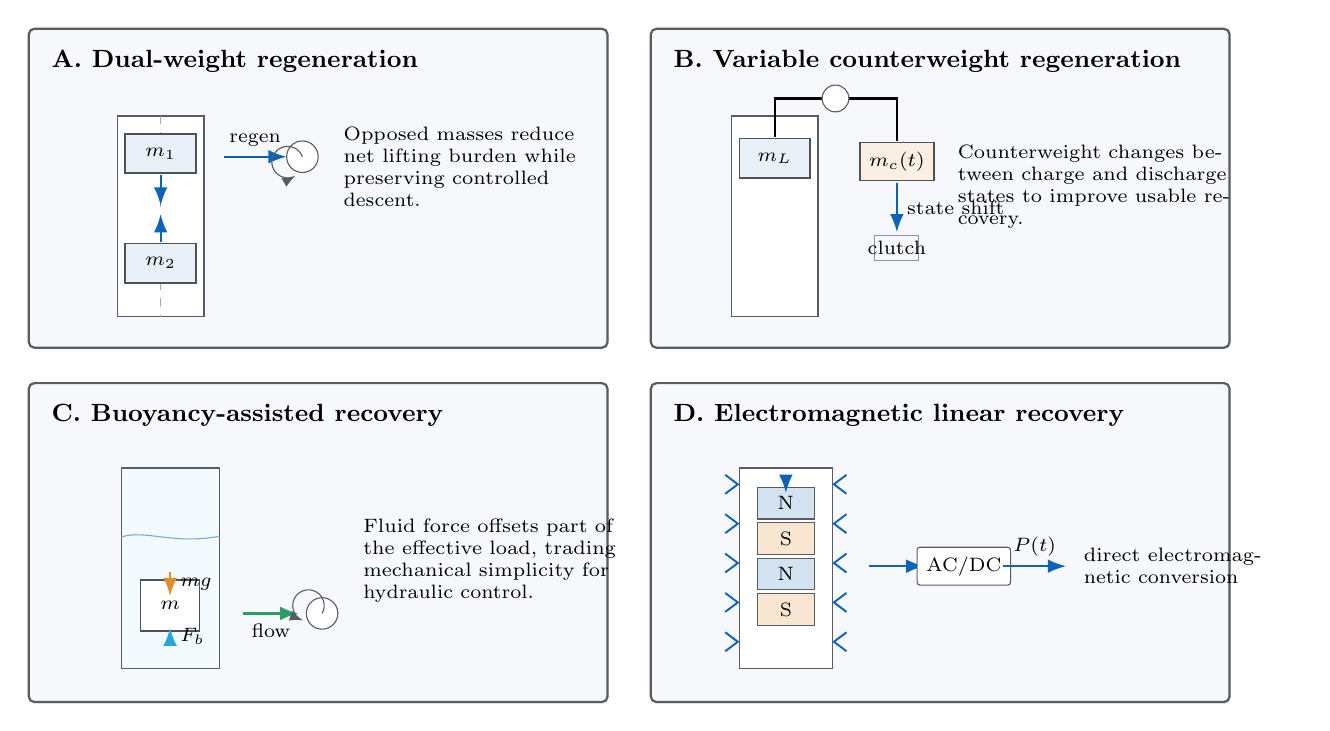
\begin{tikzpicture}[font=\scriptsize,>=Latex]
\tikzset{
  box/.style={rounded corners=2pt,draw=ink!70,fill=panel,thick,minimum width=7.35cm,minimum height=4.05cm,drop shadow={shadow xshift=0.45pt,shadow yshift=-0.55pt,opacity=0.16}},
  shaft/.style={draw=ink!70,fill=white,line width=0.55pt},
  mass/.style={draw=ink!75,fill=darkpanel,line width=0.6pt},
  coil/.style={draw=blueprint,line width=0.7pt},
  flow/.style={->,line width=0.8pt,draw=blueprint}
}
\node[box] (A) at (0,0) {};
\node[box] (B) at (7.9,0) {};
\node[box] (C) at (0,-4.5) {};
\node[box] (D) at (7.9,-4.5) {};
\node[anchor=north west,font=\bfseries\small] at ($(A.north west)+(0.18,-0.16)$) {A. Dual-weight regeneration};
\node[anchor=north west,font=\bfseries\small] at ($(B.north west)+(0.18,-0.16)$) {B. Variable counterweight regeneration};
\node[anchor=north west,font=\bfseries\small] at ($(C.north west)+(0.18,-0.16)$) {C. Buoyancy-assisted recovery};
\node[anchor=north west,font=\bfseries\small] at ($(D.north west)+(0.18,-0.16)$) {D. Electromagnetic linear recovery};

\begin{scope}[shift={(-2.55,-0.28)}]
\draw[shaft] (0,1.2) rectangle (1.1,-1.35);
\draw[muted!55,dashed] (0.55,1.2)--(0.55,-1.35);
\node[mass,minimum width=0.9cm,minimum height=0.5cm] (m1) at (0.55,0.72) {$m_1$};
\node[mass,minimum width=0.9cm,minimum height=0.5cm] (m2) at (0.55,-0.67) {$m_2$};
\draw[flow] (1.35,0.68)--(2.15,0.68) node[midway,above] {regen};
\draw[draw=ink!70,fill=white] (2.35,0.68) circle (0.2);
\draw[->,draw=ink!70] (2.35,0.68) arc(20:300:0.2);
\node[align=left,anchor=west,text width=3.1cm] at (2.75,0.55) {Opposed masses reduce net lifting burden while preserving controlled descent.};
\draw[flow] (0.55,0.45)--(0.55,0.06);
\draw[flow] (0.55,-0.4)--(0.55,-0.05);
\end{scope}

\begin{scope}[shift={(5.25,-0.28)}]
\draw[shaft] (0,1.2) rectangle (1.1,-1.35);
\node[mass,minimum width=0.9cm,minimum height=0.5cm] at (0.55,0.66) {$m_L$};
\draw[thick] (0.55,0.93)--(0.55,1.42)--(2.1,1.42)--(2.1,0.88);
\node[mass,minimum width=0.82cm,minimum height=0.46cm,fill=orange!14] at (2.1,0.62) {$m_c(t)$};
\draw[draw=ink!70,fill=white] (1.32,1.42) circle (0.17);
\node[align=left,anchor=west,text width=3.45cm] at (2.75,0.3) {Counterweight changes between charge and discharge states to improve usable recovery.};
\draw[flow] (2.1,0.35)--(2.1,-0.28) node[midway,right] {state shift};
\draw[muted!70] (1.82,-0.32) rectangle (2.38,-0.64);
\node at (2.1,-0.48) {clutch};
\end{scope}

\begin{scope}[shift={(-2.5,-4.75)}]
\draw[shaft,fill=cyan!6] (0,1.2) rectangle (1.25,-1.35);
\draw[blueprint!55] (0,0.32).. controls (0.3,0.42) and (0.65,0.22).. (1.25,0.33);
\node[mass,minimum width=0.75cm,minimum height=0.65cm,fill=white] at (0.62,-0.55) {$m$};
\draw[flow,draw=green] (1.55,-0.65)--(2.25,-0.65) node[midway,below] {flow};
\draw[draw=ink!70,fill=white] (2.55,-0.65) circle (0.2);
\draw[->,draw=ink!70] (2.55,-0.65) arc(-30:250:0.2);
\node[align=left,anchor=west,text width=3.25cm] at (2.95,0.02) {Fluid force offsets part of the effective load, trading mechanical simplicity for hydraulic control.};
\draw[->,draw=cyan,line width=0.8pt] (0.62,-1.05)--(0.62,-0.83) node[midway,right] {$F_b$};
\draw[->,draw=orange,line width=0.8pt] (0.62,-0.13)--(0.62,-0.43) node[midway,right] {$mg$};
\end{scope}

\begin{scope}[shift={(5.35,-4.75)}]
\draw[shaft] (0,1.2) rectangle (1.18,-1.35);
\foreach \y in {0.87,0.37,-0.13,-0.63,-1.13} {
  \draw[coil] (-0.18,\y) -- (-0.02,\y+0.12) -- (-0.18,\y+0.24);
  \draw[coil] (1.36,\y) -- (1.2,\y+0.12) -- (1.36,\y+0.24);
}
\foreach \y/\lab/\col in {0.75/N/blueprint!18,0.30/S/orange!22,-0.15/N/blueprint!18,-0.60/S/orange!22} {
  \node[draw=ink!70,fill=\col,minimum width=0.72cm,minimum height=0.26cm] at (0.59,\y) {\lab};
}
\draw[flow] (1.65,-0.05)--(2.35,-0.05);
\node[draw=ink!70,fill=white,rounded corners=1pt,minimum width=1.05cm,minimum height=0.48cm] at (2.85,-0.05) {AC/DC};
\draw[flow] (3.35,-0.05)--(4.15,-0.05) node[midway,above] {$P(t)$};
\node[align=left,anchor=west,text width=2.65cm] at (4.25,-0.05) {direct electromagnetic conversion};
\draw[flow] (0.59,1.05)--(0.59,0.88);
\end{scope}
\end{tikzpicture}}
\caption{Provisional four-architecture overview. This figure is meant to show the final level of diagram quality and not to claim these provisional mechanisms are the final project.}
\label{fig:quad}
\end{figure}

\clearpage
% ---------------- Page 3 ----------------
\section{Electromagnetic Linear Generator Subsystem}
The electromagnetic architecture is the best candidate for a complex research-paper diagram because it contains a complete electromechanical chain: translator motion, magnetic flux linkage, coils, air gap, guide rails, converter, controller, and load. It should be the most detailed subsystem even if the final project emphasizes the four-system comparison.

\begin{figure}[H]
\centering
\resizebox{0.98\textwidth}{!}{%
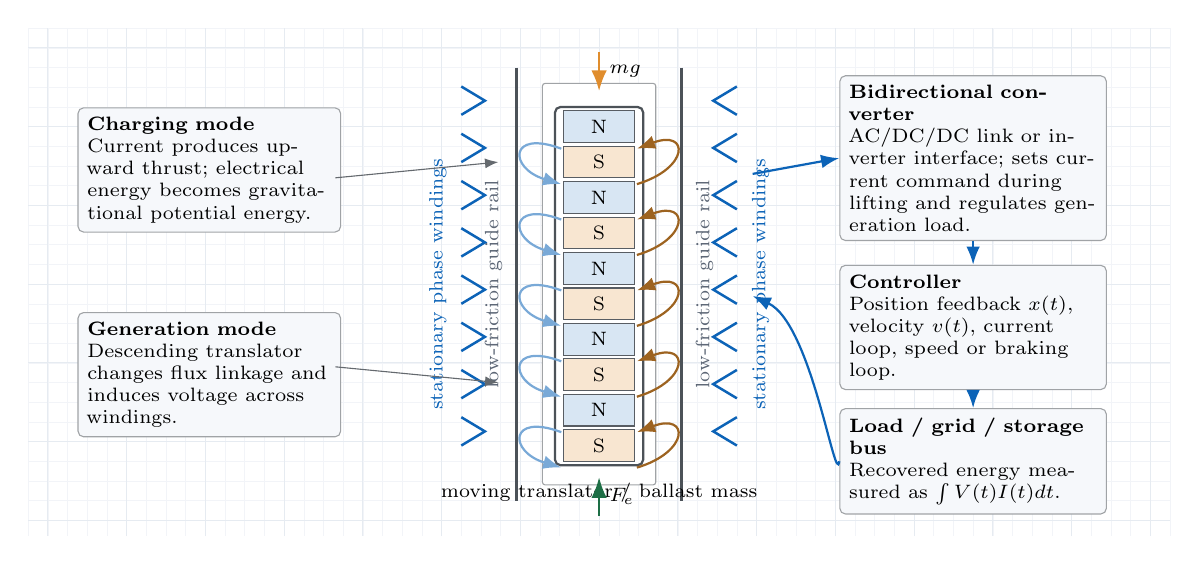
\begin{tikzpicture}[font=\scriptsize,>=Latex]
\tikzset{coil/.style={draw=blueprint,line width=0.9pt}, rail/.style={draw=ink!75,line width=1.0pt}, magN/.style={draw=ink!70,fill=blueprint!16}, magS/.style={draw=ink!70,fill=orange!22}, note/.style={draw=ink!40,fill=panel,rounded corners=2pt,align=left}}
\begin{scope}[on background layer]
\draw[step=0.25,gridgray!35,very thin] (-7.25,-3.2) grid (7.25,3.25);
\draw[step=1.0,gridgray!65,thin] (-7.25,-3.2) grid (7.25,3.25);
\end{scope}
\draw[rail] (-1.05,2.75)--(-1.05,-2.75);
\draw[rail] (1.05,2.75)--(1.05,-2.75);
\draw[draw=ink!40,fill=white,rounded corners=1pt] (-0.72,2.55) rectangle (0.72,-2.55);
\node[rotate=90,muted] at (-1.34,0) {low-friction guide rail};
\node[rotate=90,muted] at (1.34,0) {low-friction guide rail};
\foreach \y in {2.15,1.55,0.95,0.35,-0.25,-0.85,-1.45,-2.05} {
  \draw[coil] (-1.75,\y) -- (-1.45,\y+0.18) -- (-1.75,\y+0.36);
  \draw[coil] (1.75,\y) -- (1.45,\y+0.18) -- (1.75,\y+0.36);
}
\node[blueprint,rotate=90] at (-2.05,0) {stationary phase windings};
\node[blueprint,rotate=90] at (2.05,0) {stationary phase windings};
\foreach \y/\pol/\style in {2.0/N/magN,1.55/S/magS,1.10/N/magN,0.65/S/magS,0.20/N/magN,-0.25/S/magS,-0.70/N/magN,-1.15/S/magS,-1.60/N/magN,-2.05/S/magS} {
  \node[\style,minimum width=0.9cm,minimum height=0.32cm] at (0,\y) {\pol};
}
\draw[draw=ink!75,line width=0.8pt,rounded corners=2pt] (-0.56,2.25) rectangle (0.56,-2.3);
\node[align=center] at (0,-2.65) {moving translator / ballast mass};
\draw[->,draw=orange,line width=1.0pt] (0,2.95)--(0,2.45) node[midway,right] {$mg$};
\draw[->,draw=green!70!black,line width=1.0pt] (0,-2.95)--(0,-2.45) node[midway,right] {$F_e$};
\foreach \y in {1.72,0.82,-0.08,-0.98,-1.88} {
  \draw[blueprint!55,thick,->] (-0.48,\y) .. controls (-1.15,\y+0.25) and (-1.15,\y-0.25) .. (-0.48,\y-0.45);
  \draw[orange!70!black,thick,->] (0.48,\y-0.45) .. controls (1.15,\y-0.25) and (1.15,\y+0.25) .. (0.48,\y);
}
\node[note,text width=3.15cm] (conv) at (4.75,1.6) {\textbf{Bidirectional converter}\\AC/DC/DC link or inverter interface; sets current command during lifting and regulates generation load.};
\node[note,text width=3.15cm] (ctrl) at (4.75,-0.55) {\textbf{Controller}\\Position feedback $x(t)$, velocity $v(t)$, current loop, speed or braking loop.};
\node[note,text width=3.15cm] (load) at (4.75,-2.25) {\textbf{Load / grid / storage bus}\\Recovered energy measured as $\int V(t)I(t)dt$.};
\draw[->,thick,draw=blueprint] (1.95,1.4)--(conv.west);
\draw[->,thick,draw=blueprint] (conv)--(ctrl);
\draw[->,thick,draw=blueprint] (ctrl)--(load);
\draw[->,thick,draw=blueprint] (load.west) .. controls (3.0,-2.6) and (2.7,-0.5) .. (1.95,-0.15);
\node[note,text width=3.1cm] at (-4.95,1.45) {\textbf{Charging mode}\\Current produces upward thrust; electrical energy becomes gravitational potential energy.};
\node[note,text width=3.1cm] at (-4.95,-1.15) {\textbf{Generation mode}\\Descending translator changes flux linkage and induces voltage across windings.};
\draw[->,draw=ink!65] (-3.35,1.35)--(-1.28,1.55);
\draw[->,draw=ink!65] (-3.35,-1.05)--(-1.28,-1.25);
\end{tikzpicture}}
\caption{Detailed concept diagram of an electromagnetic gravity battery subsystem. Replace the translator, coil, and converter geometry with the actual final design.}
\label{fig:em}
\end{figure}

\subsection{Governing Relations}
For a translator of mass $m_T$ moving vertically with velocity $v$, a simple vertical motion model is
\begin{equation}
M\frac{dv}{dt}=F_e-mg-Bv-F_f-F_{brake},
\label{eq:dyn}
\end{equation}
where $F_e$ is electromagnetic thrust, $Bv$ is viscous loss, $F_f$ is dry friction or guide-rail loss, and $F_{brake}$ is controlled braking. During generation, $F_e$ opposes descent and extracts electrical power. A simplified induced-voltage relationship is
\begin{equation}
\mathcal{E}(t)=-N\frac{d\Phi(x)}{dt}=-N\frac{d\Phi}{dx}\frac{dx}{dt}.
\label{eq:faraday}
\end{equation}
These equations are enough for a student paper to explain why mass, height, speed, magnet spacing, coil turns, air gap, and friction matter.

\clearpage
% ---------------- Page 4 ----------------
\section{Control and Prototype Integration}
A credible paper should show how the system is controlled and how a prototype collects data. Even if the final prototype is mechanical rather than electromagnetic, the same structure applies: command, actuator/generator, mass motion, feedback, and measured electrical output.

\begin{figure}[H]
\centering
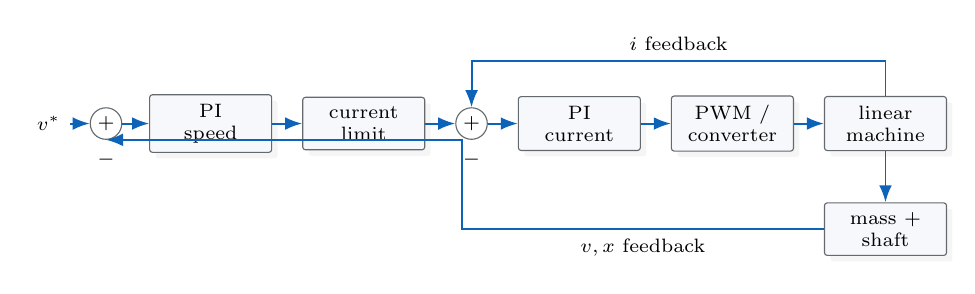
\begin{tikzpicture}[font=\scriptsize,>=Latex,node distance=0.38cm]
\tikzset{block/.style={draw=ink!65,fill=panel,rounded corners=1pt,minimum width=1.55cm,minimum height=0.6cm,align=center,drop shadow={opacity=0.08}}, sum/.style={draw=ink!65,circle,inner sep=1.2pt,fill=white}, arr/.style={->,draw=blueprint,line width=0.7pt}}
\node (r) {$v^*$};
\node[sum,right=0.25cm of r] (s1) {$+$};
\node[block,right=0.34cm of s1] (spd) {PI\\speed};
\node[block,right=0.38cm of spd] (ilim) {current\\limit};
\node[sum,right=0.38cm of ilim] (s2) {$+$};
\node[block,right=0.38cm of s2] (cur) {PI\\current};
\node[block,right=0.38cm of cur] (inv) {PWM /\\converter};
\node[block,right=0.38cm of inv] (lem) {linear\\machine};
\node[block,below=0.65cm of lem] (mech) {mass +\\shaft};
\draw[arr] (r)--(s1); \draw[arr] (s1)--(spd); \draw[arr] (spd)--(ilim); \draw[arr] (ilim)--(s2); \draw[arr] (s2)--(cur); \draw[arr] (cur)--(inv); \draw[arr] (inv)--(lem); \draw[arr] (lem)--(mech);
\draw[arr] (mech.west) -- ++(-4.6,0) node[midway,below] {$v,x$ feedback} |- (s1.south);
\draw[arr] (lem.north) -- ++(0,0.45) -| (s2.north) node[pos=0.25,above] {$i$ feedback};
\node[below=0.04cm of s1] {$-$};
\node[below=0.04cm of s2] {$-$};
\end{tikzpicture}
\caption{Generic cascaded speed-current controller for a linear-machine gravity storage subsystem.}
\label{fig:control}
\end{figure}

\begin{figure}[H]
\centering
\resizebox{0.76\textwidth}{!}{%
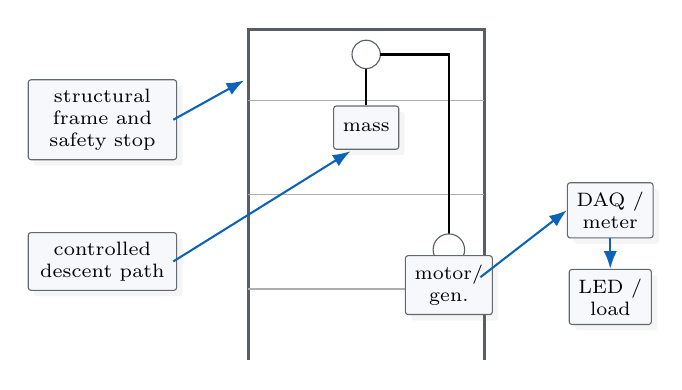
\begin{tikzpicture}[font=\scriptsize,>=Latex]
\tikzset{part/.style={draw=ink!65,fill=panel,rounded corners=1pt,align=center,drop shadow={opacity=0.08}}, arr/.style={->,draw=blueprint,line width=0.75pt}}
\draw[draw=ink!70,line width=1.1pt] (-1.5,-2.1)--(-1.5,2.1)--(1.5,2.1)--(1.5,-2.1);
\draw[draw=ink!35] (-1.5,1.2)--(1.5,1.2);
\draw[draw=ink!35] (-1.5,0.0)--(1.5,0.0);
\draw[draw=ink!35] (-1.5,-1.2)--(1.5,-1.2);
\node[part,minimum width=0.75cm,minimum height=0.55cm] (w) at (0,0.85) {mass};
\draw[thick] (w.north)--(0,1.78);
\draw[draw=ink!70,fill=white] (0,1.78) circle (0.18);
\draw[thick] (0.18,1.78)--(1.05,1.78)--(1.05,-0.5);
\draw[draw=ink!70,fill=white] (1.05,-0.7) circle (0.2);
\node[part,minimum width=0.8cm] at (1.05,-1.15) {motor/\\gen.};
\node[part,minimum width=1.05cm] (meter) at (3.1,-0.2) {DAQ /\\meter};
\node[part,minimum width=0.92cm] (load) at (3.1,-1.3) {LED /\\load};
\draw[arr] (1.45,-1.05)--(meter.west);
\draw[arr] (meter)--(load);
\node[part,text width=1.65cm] at (-3.35,0.95) {structural frame and safety stop};
\node[part,text width=1.65cm] at (-3.35,-0.85) {controlled descent path};
\draw[arr] (-2.45,0.95)--(-1.55,1.45);
\draw[arr] (-2.45,-0.85)--(-0.2,0.55);
\end{tikzpicture}}
\caption{Prototype-as-testbed diagram. Replace with actual dimensions, generator model, masses, sensors, and measured outputs.}
\label{fig:proto}
\end{figure}

\section{Placeholder Simulation and Results Format}
The comparison assumes a common baseline only for demonstration:
\begin{equation}
\mathcal{B}=\{m=\SI{50}{kg},\ \Delta h=\SI{3}{m},\ g=\SI{9.81}{m/s^2}\},\qquad E_g=\SI{1471.5}{J}.
\end{equation}
Recovered energy should be calculated from electrical measurement:
\begin{equation}
E_{out}=\int_{t_0}^{t_1}V(t)I(t)\,dt,\qquad \eta=\frac{E_{out}}{E_{in}}.
\end{equation}

\clearpage
% ---------------- Page 5 ----------------
\section{Comparison Figures for Final Data}
The final paper should avoid paragraphs of vague claims. Instead, it should show a compact comparison table and at least two plots: a system-level performance chart and a time-domain output curve.

\begin{table}[H]
\centering
\caption{Demonstration-only architecture comparison. Replace with final data.}
\label{tab:comparison}
\small
\begin{tabularx}{0.95\textwidth}{@{}lccX@{}}
\toprule
Architecture & Placeholder $\eta$ & Complexity & Primary limitation \\
\midrule
Dual-weight regeneration & 0.52 & Medium & balancing and synchronization of opposed masses \\
Variable counterweight & 0.77 & Medium-High & switching mechanism, clutch timing, safety \\
Buoyancy-assisted recovery & 0.44 & High & leakage, seals, pump losses, hydraulic drag \\
Electromagnetic linear recovery & 0.27 & High & air gap, copper losses, magnet cost, control complexity \\
\bottomrule
\end{tabularx}
\end{table}

\begin{figure}[H]
\centering
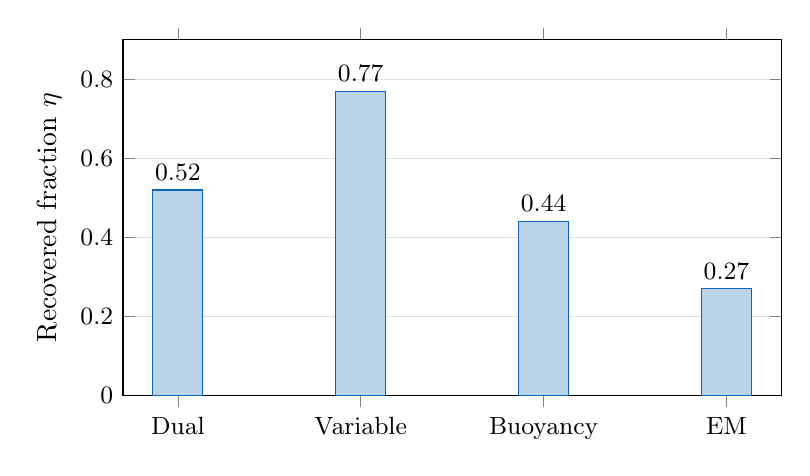
\begin{tikzpicture}
\begin{axis}[
width=0.82\textwidth,height=6.1cm,
ybar,bar width=18pt,
ymin=0,ymax=0.9,
ylabel={Recovered fraction $\eta$},
symbolic x coords={Dual,Variable,Buoyancy,EM},
xtick=data,
xticklabel style={font=\small},
yticklabel style={font=\small},
ymajorgrids=true,grid style={gridgray},
nodes near coords,
nodes near coords style={font=\small,/pgf/number format/.cd,fixed,precision=2},
]
\addplot[fill=blueprint!28,draw=blueprint] coordinates {(Dual,0.52) (Variable,0.77) (Buoyancy,0.44) (EM,0.27)};
\end{axis}
\end{tikzpicture}
\caption{Placeholder efficiency comparison across four architectures. The current values are visual placeholders only.}
\label{fig:bars}
\end{figure}

\begin{figure}[H]
\centering
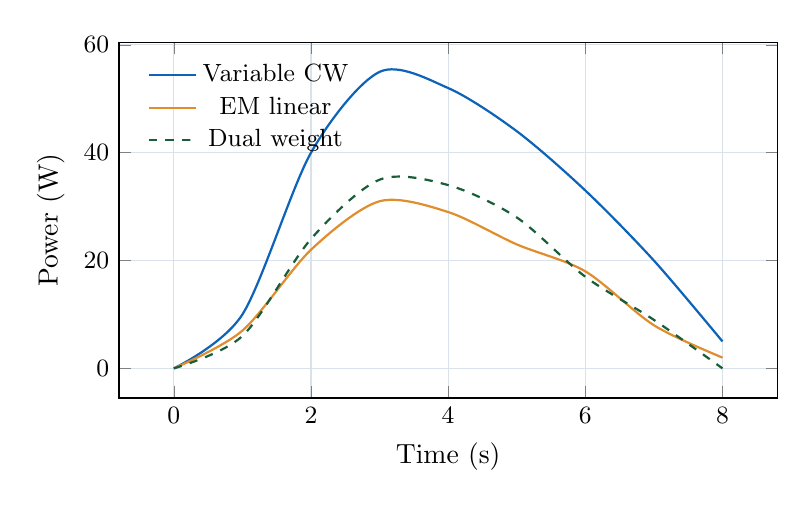
\begin{tikzpicture}
\begin{axis}[
width=0.82\textwidth,height=6.1cm,
xlabel={Time (s)},ylabel={Power (W)},
legend style={font=\small,at={(0.03,0.97)},anchor=north west,draw=none,fill=none},
xticklabel style={font=\small},yticklabel style={font=\small},
ymajorgrids=true,xmajorgrids=true,grid style={gridgray},
]
\addplot[blueprint,thick,smooth] coordinates {(0,0)(1,10)(2,40)(3,55)(4,52)(5,44)(6,33)(7,20)(8,5)};
\addlegendentry{Variable CW}
\addplot[orange,thick,smooth] coordinates {(0,0)(1,7)(2,22)(3,31)(4,29)(5,23)(6,18)(7,8)(8,2)};
\addlegendentry{EM linear}
\addplot[green!60!black,thick,smooth,dashed] coordinates {(0,0)(1,6)(2,24)(3,35)(4,34)(5,28)(6,17)(7,9)(8,0)};
\addlegendentry{Dual weight}
\end{axis}
\end{tikzpicture}
\caption{Example discharge-power curves for a future results section. Replace with measured voltage-current integration.}
\label{fig:power}
\end{figure}

\clearpage
% ---------------- Page 6 ----------------
\section{Originality and Final Manuscript Strategy}
The strongest final paper should explicitly distinguish between prior art and student contribution. The electromagnetic system can look the most advanced on paper, but it is also the closest to existing linear-machine GES literature. Therefore, the safest final framing is:

\begin{tcolorbox}[enhanced,colback=blueprint!5,colframe=blueprint,boxrule=0.75pt,arc=2pt]
\textbf{Defensible originality claim:} the project develops and compares four gravity-regeneration architectures under common constraints, then uses prototype and simulation data to identify the most practical architecture for student-scale and infrastructure-scale applications.
\end{tcolorbox}

\begin{table}[H]
\centering
\caption{Suggested prior-art positioning for the final paper.}
\label{tab:prior}
\small
\begin{tabularx}{0.95\textwidth}{@{}p{0.28\textwidth}X@{}}
\toprule
Prior-art category & Difference to emphasize \\
\midrule
Pumped hydro & Uses fluid elevation at geographic scale; project explores dry and modular vertical systems. \\
Dry gravity towers & Usually grid-scale and single-architecture; project compares four alternatives. \\
Linear-machine GES & Prior art validates electromagnetic pathway; project treats EM as one system in a comparative family. \\
Educational gravity demos & Usually show falling-weight generation only; project adds architecture-level analysis and regeneration comparison. \\
\bottomrule
\end{tabularx}
\end{table}

\section{Conclusion}
This demonstration manuscript shows the intended level of polish for a final research-style appendix: technical diagrams, equations, block diagrams, tables, and plots. The electromagnetic system deserves the most detailed figure because it supports direct electromechanical modeling and looks closest to a real engineering paper. However, the full four-system comparison is likely stronger for an invention competition because it shows ideation, originality research, design choices, testing strategy, and refinement across multiple possible solutions.

\section*{Acknowledgment}
This draft intentionally contains placeholder values and provisional mechanisms. The final version should cite the student's logbook, prototype photographs, measured data, MATLAB files, expert feedback, and the specific research papers used for originality research.

\begin{thebibliography}{9}\small
\bibitem{mugyema2022} M. Mugyema, M. M. Rabadia, C. D. Botha, M. J. Kamper, and R.-J. Wang, ``Design and Control of a Linear Electric Machine Based Gravity Energy Storage System,'' \textit{2022 SAUPEC Conference}, Durban, South Africa, Jan. 2022.
\bibitem{botha2019} C. Botha and M. Kamper, ``Capability study of dry gravity energy storage,'' \textit{Journal of Energy Storage}, vol. 23, pp. 159--174, 2019.
\bibitem{placeholder} Student inventor logbook, prototype notes, and simulation files, to be inserted in final manuscript.
\end{thebibliography}

\end{document}
